\documentclass[]{article}
\setlength{\parskip=0.7}{\baselineskip}
\setlength{\parindent}{0pt}

\usepackage{times}
\usepackage{fullpage}

\usepackage{epsfig}
\usepackage{subfigure}

\usepackage{listings}
\usepackage{siunitx}
\usepackage[super]{nth}

\usepackage[sharp]{easylist}

\usepackage[table,xcdraw]{xcolor}

\definecolor{NavyBlue}{cmyk}{0.94,0.54,0,0.5}
\definecolor{BrickRed}{cmyk}{0.16,0.89,0.61,0.2}
\usepackage{url}
\usepackage{breakurl}

\usepackage[
        colorlinks=true,
        urlcolor=NavyBlue, 
        linkcolor=NavyBlue, 
        bookmarksopen=true]{hyperref}
\hypersetup{
    colorlinks,citecolor=NavyBlue,
    linkcolor={red!50!black},
    urlcolor={blue!90!black}
}


\newcommand{\us}{$\mu$s }
\newcommand{\subtopic}[1]{\vspace{1.5pt} \noindent \textbf{#1}}

\definecolor{notecolor}{rgb}{0.75,0,0} % A darker red
\newcommand{\todo}[1]{\textcolor{notecolor}{\textbf{TODO: #1}}}
\newcommand{\hl}[1]{\textcolor{notecolor}{#1}}
\newcommand{\fixit}[2][]{\textcolor{notecolor}{%
     \ifthenelse{\isempty{#1}}{\textbf{[Fixit: %
         #2]}}{\textbf{#2\footnote{\textcolor{notecolor}{Fixit: #1}}}}}}
\newenvironment{highlight}{\par\color{notecolor}}{\par}





\begin{document}

\title{Kawkab: A Distributed Filesystem for Fast Data}
%\author{Sajjad Rizvi, Bernard Wong}
\date{}
\maketitle

\bgroup
\def\arraystretch{1.5}
\begin{table}[!htb]
\centering
\caption{Change Log}
\label{table:change-log}
\begin{tabular}{|l|l|l|}
\hline
\rowcolor[HTML]{EFEFEF} 
Date             & Description  & Participants  \\ \hline
 March 03, 2017  & Kawkab single node design           & Sajjad  \\ \hline
 March 10, 2017  & - Added sections 3 and 4, about the distributed design of Kawkab& \\ 
                 & - Updated architecture diagram & Sajjad  \\ \hline
\end{tabular}
\end{table}
\egroup


\section{Introduction} Kawkab is a distributed filsesystem developed to
efficiently manage large amounts of streaming data.

\section{Architecture} 

\begin{figure}[t]
    \centering
    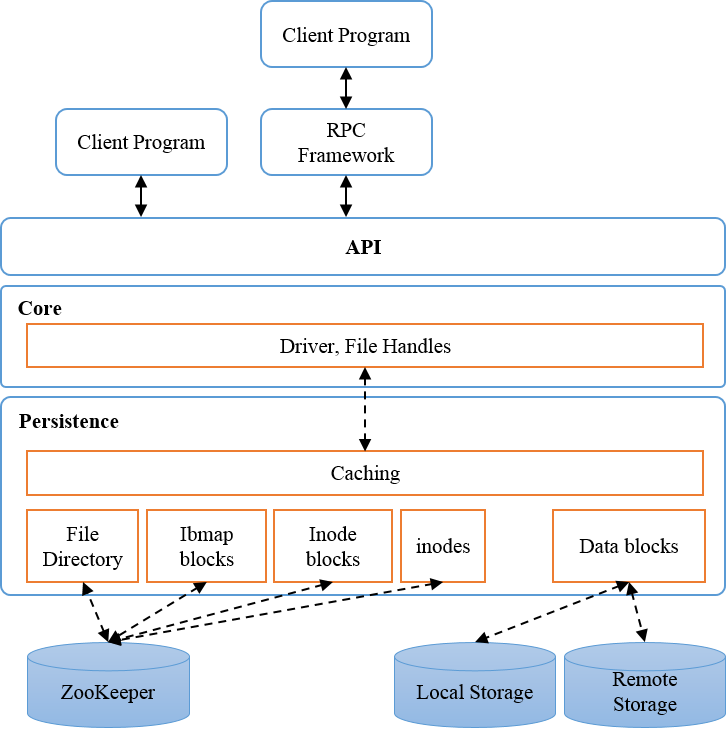
\includegraphics[width=0.55\columnwidth]{{figures/architecture.png}}
    \caption{Kawkab architecture.}
   \label{fig:architecture}
\end{figure}

Kawkab mainly follows the design approach of a standard
Unix filesystem. The reasons to follow the Unix filesystem is to control the
memory usage of the system and make the system memory efficient.

The system is divided in three layers: API layer, core, and persistence.
Clients interact with the API layer directly or using an RPC service.  API
provides functions to open, close, read, and write files through the core
layer.

The core layer controls the metadata of the whole system. It mainly consists of
four structures: a file directory, an index node bitmap, index nodes, and data
blocks. Only the data blocks contain the actual data of a file. The other
structures comprise the metadata of the filesystem.

\subsection{Storage Space Design}

\begin{figure}[t]
    \centering
    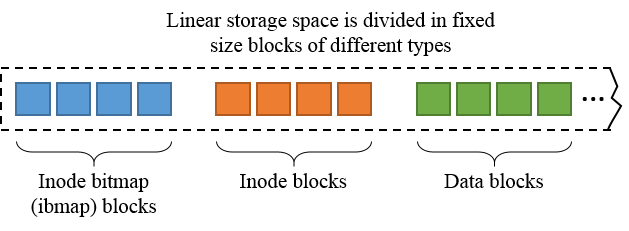
\includegraphics[width=0.5\columnwidth]{{figures/linear-space.png}}
    \caption{Filesystem is designed as a very large storage space organized in fixed size blocks.}
   \label{fig:storage-space}
\end{figure}

\begin{figure}[t]
    \centering
    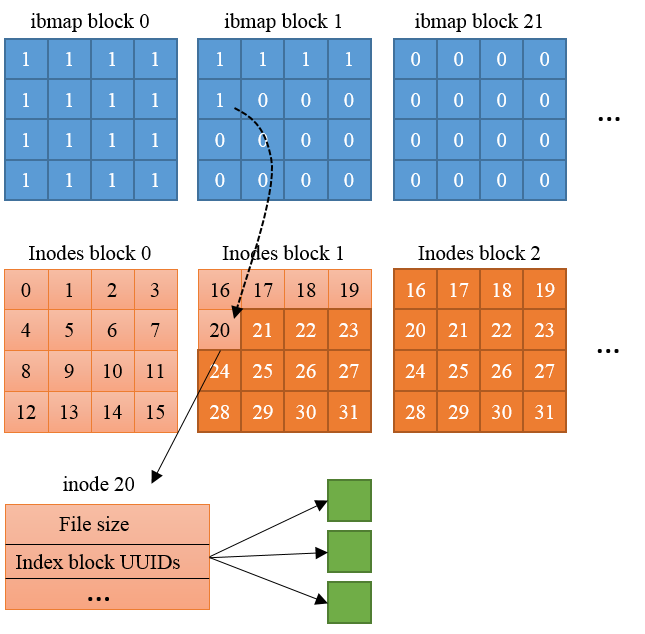
\includegraphics[width=0.5\columnwidth]{{figures/blocks-layout.png}}
    \caption{Layout of different types of blocks.}
   \label{fig:blocks-layout}
\end{figure}



The system is designed such that the files are stored in a very large linear
storage space. The storage space is a collection of fixed size blocks $\{B_1,
B_2, \ldots, B_N\}$.  Each block has a unique ID (UUID), and the blocks are
persistently stored as files on the local storage devices (HDDs, SSDs) and the
cloud, e.g., Amazon EB3 and S3.

The blocks in the storage space are of three types: index node bitmap blocks,
index-node blocks, and data blocks.

\subtopic{Data blocks:} The data blocks contains the actual data belonging to
the files in the system. However, to associate the blocks with a file, the
blocks are indexed using a structure called \textit{index node} or
\textit{inode}. Thus, a file in Kawkab consists of an inode and a collection of
data blocks. The inode, which is further explained in the section~\ref{},
contains the metadata of the file and the IDs of the data blocks belonging
to the file. 

An inode is uniquely referred through a number called \textit{inumber}.
Moreover, an inode is a fixed size structure, and it is stored in an
\textit{index-node block} of our linear storage device.

\subtopic{Index-nodes blocks:} An index-nodes block, or \textit{inode block},
is a fixed size block that contains a predefined number of \textit{inodes}.
%The maximum number of inode blocks in the system controls the maximum number
%of files supported in the system because the filesystem has a fixed number of
%inode blocks.  As the filesystem has fixed number of inode blocks, which also
%controls the number of files supported by the system.
As each inode has a fixed size $S_I$ bytes, an inode block $B$ contains $N =
S_{B} / S_I$ number of inodes, where $S_B$ is the size of an inodes block.
Thus, the inode number $x$ is located in the inode block number $ x / N$. In
this way, given an inode number, Kawkab can calculate the inode block that
contains the inode, and the index of the inode in the block.

When a file is created, the file is assigned a unique inumber, which
is the first available inode number in the system. To achieve that, the
system keeps track of the inumbers already assigned using a bitmap
called \textit{inode bitmap} or \textit{ibmap}. The ibmap is stored in
the blocks of type "inode bitmap block".


\subtopic{Inode Bitmap Blocks:} An inode bitmap block, or ibmap block,
is a fixed size block that contains part of the ibmap. 
Each bit at index $i$ in the ibmap indicates whether the inode of inumber $i$ 
is already used or not. 

When a new file is created, Kawkab scans the ibmap to find the first unused 
inumber and assigns that inumber to the inode associated with the file. Moreover,
Kawkab sets the bit in the bitmap that is associated with the inumber.
When a file is deleted, Kawkab clears the bit in the ibmap, which allows
Kawkab to reuse the inode and the inumber for the next new file.


\subsection{File Directory} Kawkab filesystem contains a file directory that
defines the namespace of the system.
%The file directory keeps track of the existing files in the system and the way
%to access the files.
Each file in the system has a unique name and a unique inode number.  The file
directory is a simple collection of $\langle$ file name, inode number $\rangle$
pairs that maps a file name to an inode number.  The clients refer to a file
using the file name whereas the system access the files through the inode
numbers. 

The file directory is the only structure that keeps the mapping of the file
names and the inode numbers. Therefore, the file directory is made persistent
and consistent through a distributed key-value store such as ZooKeeper.

\subtopic{File Namespace:} Kawkab has a flat namespace. Kawkab does not maintain
directory hierarchies. However, a user can use any file name.



\subsection{Index Node} An index node, called \textit{inode}, is the main
structure that keeps track of the file metadata and IDs of the data
blocks associated with the file. An inode is a fixed size structure that
consists of the following parts:

\begin{enumerate}
  \item \subtopic{File Metadata:} The file metadata consists of information
        about the file such as file creation time, last access time, file
        rights, and file size.

	\item \subtopic{First $N$ Data Blocks:} An inode contains a fixed number
$N$ of the IDs of the first $N$ data blocks associated with the file.
These data blocks are directly accessible from the inode and requires
only one step lookup in the inode.
%An inode keeps the reference of the first $N$ data blocks of the file. 
The number $N$ is kept small to optimize for the memory space and the file
access for smaller files. 

  \item \subtopic{Indirect Block:} 
An inode contains the ID of one indirect block, where an indirect block is
special data block that only consists of the IDs of the data blocks associated
with the file. Thus, an indirect block is level-1 index into the file.
As the size of each block is fixed, an indirect block contains the
IDs of a fixed number of data blocks in a file. These data blocks 
range from $N+1$ to $M$ where $M$ is the number of IDs stored in the
direct block.

  \item \subtopic{Double and Triple Indirect Block:}
An inode has one double and one triple indirect block. A double indirect block is a two
level index, i.e., a double indirect block is the ID of a special data block that contains
the IDs of indirect blocks. Similarly, a triple indirect block contains the IDs of the
double indirect blocks. These indexing levels are sufficient to support the maximum 
file size in Kawkab, which is $2^{63}-1$ bytes.

\end{enumerate}

\subsection{Data Blocks} Kawkab has fixed size data blocks. Each data block has
a unique ID, generated as a UUID.  Each block is persistently stored as a file
in the persistent storage of the system, e.g., local or remote disks, EB3, or
S3.  The name of the persistent file is extracted from the UUID: the UUID is
converted to an ASCII character string using Base64 encoding.  The ASCII name
is then converted into a file path such that each two characters in the ASCII
representation of the UUID become a directory name in the persistent storage.
For example, a UUID \texttt{ABCDEFGH} is stored as a file
\texttt{/storage/datablocks/AB/CD/EF/GH}.


\subsection{Persistence Layer}
\hl{Note: This section is incomplete.}

The persistence layer in Kawkab keeps track of the location of each file in the system.
All the blocks are stored and retrieved from the persistence layer using the UUIDs
of the blocks.

The persistence layer has a caching sub-module. The caching module acts as an
LRU cache and controls the memory of one machine.


\subsection{Block Metadata} In order to achieve faster data access, each block
has an associated metadata that is stored along with the block's UUID. The
metadata includes: first append time, last append time, and the additional
data boundaries that allow fine grained indexing within a data block.

\subsection{Data Access and Indexing}
\hl{Note: This section is incomplete.}

Kawkab is an append-only system. Each append is performed at the end of the file.
However, a file can be read from any location. When a client opens a file,
it is returned a FileHandle. The FileHandle contains a read pointer that indicates
the current position in the file from where the data will be read. The read
pointer can be moved to any position in the file using any of the following
ways: 

\begin{enumerate}
  \item Move to an absolute byte offset in the file.
  \item Give a timestamp T:
  \begin{itemize}
    \item Move to the first byte of the closest block that has the append time equal to
          or \textit{before} T.
    \item Move to the first byte of the closest block that has the append time equal to
          or \textit{after} T.
  \end{itemize}
\end{enumerate}

In order to find the data block that contains the given byte or timestamp, Kawkab
performs binary search over the index in the inode.

TODO:

\begin{itemize}
  \item Indexing within a block
  \item Time range queries
\end{itemize}

%  - How data is indexed
% - How data is retrieved given a byte offset
 % - How data is retrieved given a timestamp

\subsection{Atomic Appends and Reading Unfinished Block}

\section{File Access Patterns}

\subtopic{File Writes:} Kawkab allows only one writer at a time to
write the file. The first client that opens the file becomes the distinguished
writer of the file. Only the distinguished writer is then allowed to append to
the file. Moreover, the node where the client is located becomes the primary
node of the file.  The other nodes may fetch recent appends from the primary
node when the data is not replicated in the cloud storage (S3/EBS).

If an existing writer fails, another client can become the distinguished writer
by successfully opening the file for writing. If the writer closes the file,
another writer can open the file and become the distinguished
writer\footnote{In the Smash's use case, files are never closed.}. However,
Kawkab allows only one file writer at a time.

Each append request consists of small number of bytes, e.g., less than 100 bytes.

\subtopic{File Reads:}
Kawkab allows multiple readers to read at the same time. If the data block
is not located locally in the system, the data block is fetched from S3/EBS if
it is available. If the data block is not available in S3/EBS, the data block
is fetched from the node where the file-writer is located.

TODO: Data access frequency and size, number of readers per node, number of
nodes where readers are located $\ldots$.



\section{Distributed Design of Kawkab}

\subsection{Distributed Metadata and Namespace}

In Kawkab, only the filesystem namespace (file directory) and other metadata
(ibmaps and inodes) are concurrently updated across the nodes. Data blocks are
not updated concurrently. Therefore, Kawkab uses a distributed key-value store
to keep to safely and consistently store the namespace, and the other metadata
is partitioned across the nodes.

\subtopic{Key-Value Store Consistency Requirements:} The basic requirement for
metadata consistency is that all of the nodes in Kawkab observe the same
sequence of updates to the file directory, the ibmaps, and the inode blocks.  
%As Kawkab allows only one file writer at a time, the indirect blocks, which
%contains the UUIDs of the data blocks and indirect blocks, do need to be made
%consistent across the nodes.
Therefore, the key-value store is required to provide at least sequential
consistency.
%The keys are file IDs and the values are the inode numbers in the key-value
%store.
We propose to use ZooKeeper because it allows conditional creation of the
nodes: an error is generated if a client tries to create an already existing
node. Moreover, ZooKeeper allows the clients to subscribe for notifications
when a node is updated.  These features can be used to maintain consistency
of the file directory across all the nodes in Kawkab.


\subsubsection{Data Blocks and Indirect Blocks} Data blocks are stored locally
on SSDs and remotely in the cloud storage such as EBS and S3. Data blocks are
not replicated to the storage of other nodes.

\subtopic{File Appends:} The file writer appends data in memory. The data
blocks are then flushed to the local SSD asynchronously for faster file write
operations. When a data block is closed, it is copied to the cloud storage.

\subtopic{File Reads:} Remote nodes read data blocks directly from the cache,
or from the cloud storage (EBS/S3) if the data blocks are not in cache.  If a
data block does not exist in the remote storage, e.g., if it is the last block
in file or the block is not yet replicated in the cloud storage, the reader
node fetches the desired block from the primary node of the file where the file
writer is located. The fetched data block is then kept in the LRU cache.

\subtopic{Indirect Blocks:} Indirect blocks, which contain the UUIDs of other
indirect blocks or data blocks, are treated the same as the data blocks.
%Indirect blocks contains UUIDs of data blocks and other indirect blocks. 
Only the file writer can update a data block or an indirect block. Therefore,
indirect blocks are stored and accessed the same was as the data blocks.


\subsubsection{Namespace Replication and Consistency}
Kawkab uses ZooKeeper to keep the namespace consistent. All the file
directory information, which consists of mappings from file IDs to the
inumbers (inode number), in ZooKeeper. ZooKeeper is a good candidate
for the namespace because the frequency of the creation of new files is low
and the higher latency for the file create operation is acceptable.

When a node creates a new file, it adds a zknode in ZooKeeper on the path
\texttt{kawkab/files/fileID} and with the node-value of the inumber assigned to
the file. If the node creation fails due to an already existing zknode with
the same path, it implies that another node has already created the file with the same
file ID. Therefore, the file opening for writing is failed. However, the file can be
opened for file reads in this situation. In this way, all the nodes view
the same file directory across the system.

The file directory is kept in cache on each node for faster file read and write
operations. Moreover, the file directory is periodically updated to reflect the
recent changes in the directory. This can be achieved by each node subscribing
to the zknode update events for \texttt{kawkab/files}.

For the file open requests in the read-only mode, first the file directory in
the cache is used to get the inumber of the file. If the file is not found in
the cache, the node reads the file from the ZooKeeper and updates the file
directory if the file is found.



\subsubsection{Ibmap and Inode-blocks Partitioning} Kawkab partitions the ibmap
and the inode blocks space across the nodes. Each node is assigned a specific
number of ibmap-blocks and the corresponding inode blocks.
%For example, N ibmap blocks and the corresponding inode blocks are assigned to
%each node. 
The blocks are assigned in a sequential order. The partitioning ensures that
each node uses a unique inumber for the new files without any synchronization
overhead.

\subtopic{Persistence:} Each node persistently stores its Ibmap blocks and the
inode blocks in its local storage as well as the remote storage. The blocks are
periodically flushed to these storage to reduce the memory and the network usage.

\subtopic{Inode Updates Across Nodes:} Inodes are frequently updated as an inode is
updated after each file append operation to reflect the changes in the file
size and the other metadata (e.g., last modified time).  Therefore, inodes need
to be made consistent across all the readers of the file.

Kawkab uses a simple publish-subscribe system to propagate the inodes' updates
across the nodes where the file-readers are located. Each node with
at least one active reader subscribes to the inode updates on the primary node
of the file, i.e., where the file writer is located. The file writer 
asynchronously publishes the inodes to all the subscribers. In this way,
the staleness of the inodes is reduced on the file readers.


\subtopic{Inodes Location from Inumbers:} It may happen that a node opens a
file for reading while the file has been created by another node. As the
location of an inode cannot be inferred from an inumber, Kawkab also stores the
mapping of the inumber range to the node location in ZooKeeper.  For example,
if $x$ inodes are assigned to each node, Kawkab stores the mappings $\langle x
\to \mathrm{node1} \rangle$, $\langle 2x \to \mathrm{node2} \rangle, \ldots$,
in the ZooKeeper, which implies that the inodes from $x$ to $2x-1$ are stored
in the node with ID $\mathrm{node1}$. As this information is static and do not
change frequently, all the nodes cache this information during bootstrap. If
the information is updated due to node failures, all the nodes are updated to
reflect the changes in their cache.



\subsection{Scalability}

\subsection{Fault-tolerance}

\subsection{Consistency Guarantees}

\subsection{Metadata and Data Journaling}

%\subtopic{Creating a New File:}
%\begin{itemize}
%  \item Get inumber \texttt{inum} from the ibmap
%  \item Execute a multi-operation transaction in ZooKeeper:
%  \begin{itemize}
%    \item Create a persistent node with path \texttt{kawkab/inodes/inum}.
%    \item Create a persistent node with path \texttt{kawkab/files/fileID} and the value equals to \texttt{inum}.
%  \end{itemize}
%  \item If the previous transaction succeeds, update the local file directory and the ibmap.
%  \item If the transaction fails, it is because either (1) The inode is already consumed, or (2) the file already
%        exists. If the file already exists, then the file creation operation returns with FileExists error. If the
%        inode is already consumed, 
%\end{itemize}


%\subsection{Distributed Namespace:}
%Kawkab partitions the namespace across all the nodes. Each node has a dedicated
%namespace, and each node creates new files in its own namespace. The metadata
%belonging to each namespace -- files directory, ibmaps, and inode blocks --
%are kept consistent across all the nodes.

%\section{File Read and Write Operations}


\section{Related Work}

\begin{easylist}[itemize]

 # Comparison with Alluxio

 # Comparison with Succinct

 # Comparison with HDFS and similar systems

\end{easylist}

\begin{figure}[t]
    \centering
    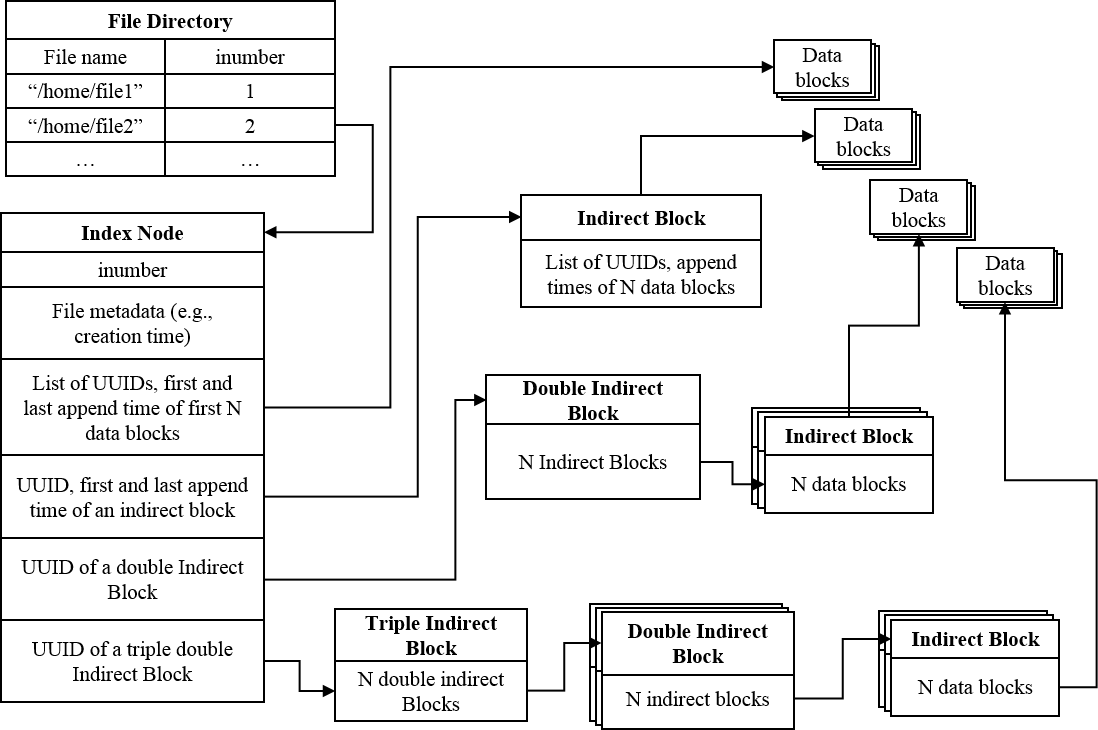
\includegraphics[width=0.9\columnwidth]{{figures/file-index-design.png}}
    \caption{File directory and file index.}
   \label{fig:data-structures}
\end{figure}



\end{document}
